\section{Cải thiện tấn công chuyển giao}
Trong tài liệu (Carlini and Wagner 2017b) đã chỉ ra rằng tấn công C\&W có khả năng chuyển giao tốt hơn  từ 1 mạng không phòng thủ sang 1 mạng phòng thủ chưng cất bằng cách tối ưu các tham số độc lập $\kappa$ trong phương trình \ref{eq:4}. Theo (Carlini and Wagner 2017b), nhóm tác giả sử dụng cùng bộ tham số của tấn công chuyển giao trên tập MNIST, vì MNIST là tập dữ liệu khó nhất khi tấn công bằng nhiễu trung bình trên mỗi ảnh như trong bảng \ref{tab:tab_2} ở trên.

Cố định $\kappa$, các mẫu đối nghịch được sinh ra từ mạng không phòng thủ gốc được sử dụng để tấn công mạng phòng thủ chưng cất với tham số nhiệt $T = 100$ (Papernot et al. 2016b). Tỷ lệ tấn công thành công (ASR) của EAD, phương pháp C\&W và I-FGM được trình bày trong hình \ref{fig:fg_04}. Khi $\kappa = 0$, tất cả các phương pháp đều cho ASR thấp và do đó không tạo được các mẫu đối nghịch có thể chuyển giao. Tỷ lệ ASR của EAD và phương pháp C\&W cải thiện khi đặt $\kappa > 0$ , trong khi đó tỷ lệ ASR của I-FGM thấp (dưới $2\%$) do tấn công không có các tham số tương tự để có thể chuyển giao.

Chú ý rằng, EAD có thể thu được ASR gần đạt $99\%$ khi $\kappa = 50$, trong khi đó ASR cao nhất mà phương pháp C\&W đạt được là gần $88\%$ khi $\kappa = 40$. Chứng tỏ rằng, khả năng chuyển giao tấn công tăng lên khi sử dụng các mẫu đối nghịch được tạo từ EAD, điều này là do thuật toán ISTA trong phương trình \ref{eq:8} mạnh hơn so với tấn công C\&W qua phương pháp shrinking and thresholding. Nhóm tác giả cũng phát hiện rằng khi đặt $\kappa$ quá lớn cũng làm giảm ASR của các tấn công chuyển giao cả bằng EAD và phương pháp C\&W, do thuật toán tối ưu không tìm được mẫu đối nghịch có thể làm tối thiểu hóa hàm mất mát $f$ trong \ref{eq:4} khi $\kappa$ lớn. Kết quả đầy đủ của việc chuyển giao tấn công được báo cáo trong tài liệu kèm theo.

\begin{figure}[H] % places figure environment here   
    \centering % Centers Graphic
    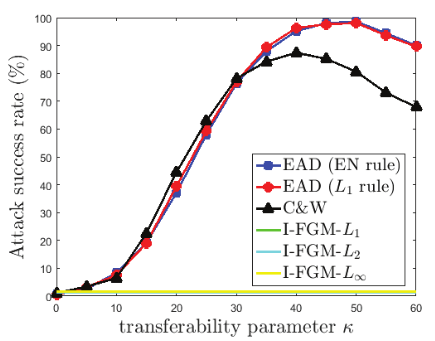
\includegraphics[width=0.5\textwidth]{assets/fig_04.png} 
    \caption{Khả năng chuyển giao tham số $\kappa$} % Creates caption  % Creates caption underneath graph
    \label{fig:fg_04}
\end{figure}